\documentclass[tikz]{standalone}%

\usepackage[utf8]{inputenx}%  http://ctan.org/pkg/inputenx
% Euler for math | Palatino for rm | Helvetica for ss | Courier for tt
\renewcommand{\rmdefault}{ppl}% rm
\linespread{1.05}% Palatino needs more leading
\usepackage[scaled]{helvet}% ss //  http://ctan.org/pkg/helvet
\usepackage{courier}% tt // http://ctan.org/pkg/courier
\usepackage{eulervm}  %  http://ctan.org/pkg/eulervm
% a better implementation of the euler package (not in gwTeX)
\normalfont%
\usepackage[T1]{fontenc}%  http://ctan.org/pkg/fontenc
\usepackage{textcomp}%  http://ctan.org/pkg/textcomp

\usetikzlibrary{patterns}

\newcommand{\bul}[1]{
  \begin{scope}[#1]
    \fill[draw = black!80, top color = black!10, bottom color = black!70]
    (0, 1mm) -- (1.5mm, 1mm) to [out = 0, in = 120] (2.5mm, 0.5mm) 
    to[out = -120, in = 0] (1.5mm, 0) -- (0, 0) -- cycle;
    \draw[white, draw opacity = 0.5] (0, 0.1mm) -- (2.3mm, 0.1mm);
  \end{scope}
}

\begin{document}
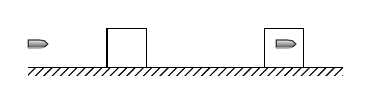
\begin{tikzpicture}
  \bul{yshift = 0.25cm}

  \draw (0, 0) coordinate (O) -- (4cm, 0);
  \draw (1cm, 0) rectangle (1.5cm, 0.5cm);

  \fill[pattern = north east lines] (O) rectangle (4cm, -0.1cm);

  \draw (3cm, 0) rectangle (3.5cm, 0.5cm);

  \bul{yshift = 0.25cm, xshift = 3.15cm}
\end{tikzpicture}
\end{document}
%%% Local Variables:
%%% mode: latex
%%% TeX-master: t
%%% End:
